\documentclass[
  bibliography=totoc,     % Literatur im Inhaltsverzeichnis
  captions=tableheading,  % Tabellenüberschriften
  titlepage=firstiscover, % Titelseite ist Deckblatt
]{scrartcl}

% Paket float verbessern
\usepackage{scrhack}

% Warnung, falls nochmal kompiliert werden muss
\usepackage[aux]{rerunfilecheck}

% deutsche Spracheinstellungen
\usepackage{polyglossia}
\setmainlanguage{german}

% unverzichtbare Mathe-Befehle
\usepackage{amsmath}
% viele Mathe-Symbole
\usepackage{amssymb}
% Erweiterungen für amsmath
\usepackage{mathtools}

% Fonteinstellungen
\usepackage{fontspec}
% Latin Modern Fonts werden automatisch geladen

\usepackage[
  math-style=ISO,    % ┐
  bold-style=ISO,    % │
  sans-style=italic, % │ ISO-Standard folgen
  nabla=upright,     % │
  partial=upright,   % ┘
  warnings-off={           % ┐
    mathtools-colon,       % │ unnötige Warnungen ausschalten
    mathtools-overbracket, % │
  },                       % ┘
]{unicode-math}

% traditionelle Fonts für Mathematik
\setmathfont{Latin Modern Math}
\setmathfont{XITS Math}[range={scr, bfscr}]
\setmathfont{XITS Math}[range={cal, bfcal}, StylisticSet=1]

% Zahlen und Einheiten
\usepackage[
  locale=DE,                 % deutsche Einstellungen
  separate-uncertainty=true, % immer Fehler mit \pm
  per-mode=reciprocal,       % ^-1 für inverse Einheiten
  output-decimal-marker=.,   % . statt , für Dezimalzahlen
]{siunitx}

% chemische Formeln
\usepackage[
  version=4,
  math-greek=default, % ┐ mit unicode-math zusammenarbeiten
  text-greek=default, % ┘
]{mhchem}

% richtige Anführungszeichen
\usepackage[autostyle]{csquotes}

% schöne Brüche im Text
\usepackage{xfrac}

% Standardplatzierung für Floats einstellen
\usepackage{float}
\floatplacement{figure}{htbp}
\floatplacement{table}{htbp}

% Floats innerhalb einer Section halten
\usepackage[
  section, % Floats innerhalb der Section halten
  below,   % unterhalb der Section aber auf der selben Seite ist ok
]{placeins}

% Seite drehen für breite Tabellen
\usepackage{pdflscape}

% Captions schöner machen.
\usepackage[
  labelfont=bf,        % Tabelle x: Abbildung y: ist jetzt fett
  font=small,          % Schrift etwas kleiner als Dokument
  width=0.9\textwidth, % maximale Breite einer Caption schmaler
]{caption}
% subfigure, subtable, subref
\usepackage{subcaption}

% Grafiken können eingebunden werden
\usepackage{graphicx}
% größere Variation von Dateinamen möglich
\usepackage{grffile}

% schöne Tabellen
\usepackage{booktabs}

% Verbesserungen am Schriftbild
\usepackage{microtype}

% Literaturverzeichnis
\usepackage[
  backend=biber,
]{biblatex}
% Quellendatenbank
\addbibresource{lit.bib}
\addbibresource{programme.bib}

% Hyperlinks im Dokument
\usepackage[
  unicode,        % Unicode in PDF-Attributen erlauben
  pdfusetitle,    % Titel, Autoren und Datum als PDF-Attribute
  pdfcreator={},  % ┐ PDF-Attribute säubern
  pdfproducer={}, % ┘
]{hyperref}
% erweiterte Bookmarks im PDF
\usepackage{bookmark}

% Trennung von Wörtern mit Strichen
\usepackage[shortcuts]{extdash}

\author{
  AUTOR A%
  \texorpdfstring{
    \\
    \href{mailto:authorA@udo.edu}{authorA@udo.edu}
  }{}%
  \texorpdfstring{\and}{, }
  AUTOR B%
  \texorpdfstring{
    \\
    \href{mailto:authorB@udo.edu}{authorB@udo.edu}
  }{}%
}
\publishers{TU Dortmund – Fakultät Physik}


\subject{Fortgeschrittenen Praktikum V14}
\title{Tomographie mittels \texorpdfstring{$\gamma$}{Gamma}-Strahlung}
\date{
  Durchführung: 25.01. 2016
  \hspace{3em}
  Abgabe: 02.02. 2016
}

\begin{document}

\maketitle
\thispagestyle{empty}
\tableofcontents
\newpage

\section{Theorie}
\label{sec:Theorie}
\footnotesize{\textit{Carl Arne Thomann}}
\cite{sample}

\section{Aufbau}
\label{sec:Aufbau}
Der Aufbau wird in Abbildung \ref{setup} gezeigt.
\begin{figure}[hp]
    \centering
    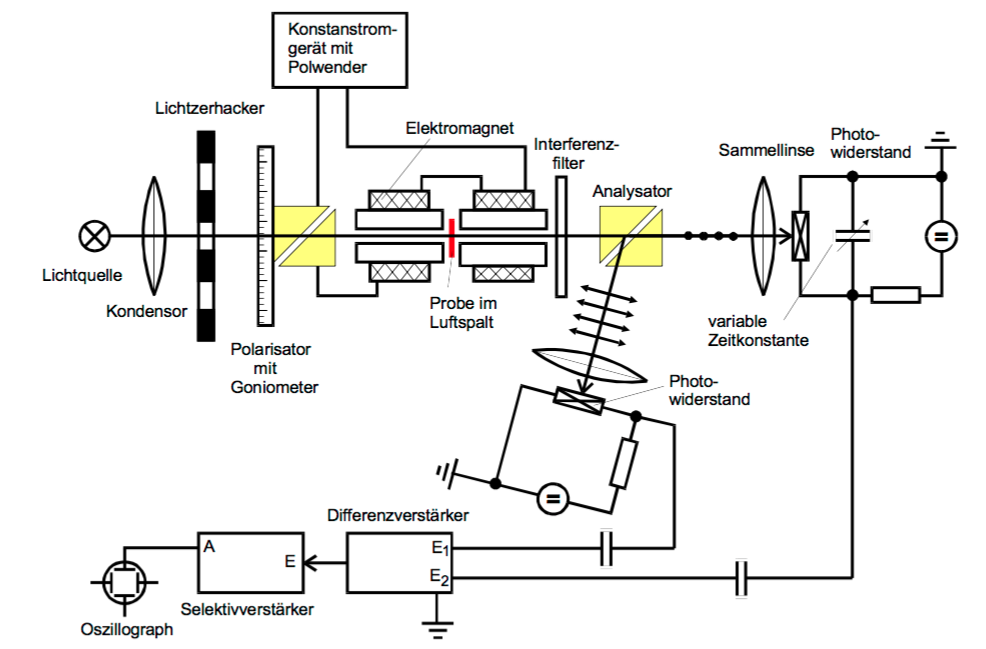
\includegraphics[width=0.9\textwidth]{graphics/setup.png}
    \caption{Trolololo \cite{skript}}
    \label{setup}
\end{figure}
Licht einer Halogenlampe fällt auf einen Interferenzfilter und Analysator,
wodurch der Strahl in zwei senkrecht zueinander linear-polarisierte Strahlen bei einer bestimmten Wellenlänge aufgespalten wird.
Die Wellenlängen-Beschränkung ist notwendig, weil die folgenden optischen Geräte für ein breites Lichtspektrum durchlässig sind,
während die Probe hauptsächlich für Infrarotes Lich durchsichtig ist.
Daher stammt Licht außerhalb vom infraroten Bereich nicht von der Probe und sollte zwecks der Messgenauigkeit gefiltert werden.
Die beiden Teilstrahlen aus dem Analysator werden auf zwei Photowiderstände fokussiert,
deren Leitfähigkeit als Maß für die Polarisationsänderung genommen werden kann.
Liegt eine Polarisation des einfallenden Lichtes vor, die in zwei gleich intensive Teile gespalten wird,
kann an den Dioden die gleiche Spannung gemessen werden.
Um den Aufwand gering zu halten, werden nicht beide Signale der Dioden, sondern die Differenz der Signale gemessen.
Es gilt entsprechend, dass ein Nullsignal eine Polarisation mit zwei gleichen (senkrechten) Polarisationsanteilen anzeigt.
Das Licht der Halogenlampe ist im Allgemeinen nicht polarisiert.
Um die Faraday-Drehung messen zu können, wird vor dem Probenhalter ein Polarimeter mit präzisem Winkelmesser (Goniometer) installiert.

Da das Experiment bei Tageslicht durchgeführt werden soll
und somit Streulicht und Rauscheffekte der Photodioden reduziert werden muss,
wird das einfallende Licht mittels Chopper zu einem Rechtecksignal einer bestimmten Frequenz moduliert.
Das Differenzsignal wird anschließend mithilfe eines Selektivverstärkers,
der auf die Frequenz des Choppers abgestimmt ist, auf diese Frequenz reduziert.

In der Mitte des Aufbaus befindet sich ein Elektromagnet, der durch seine Bauart geeignet ist,
ein starkes homogenes Feld zu erzeugen und dabei den Lichtweg nicht zu behindern.
In den Bereich des stärksten Feldes ist ein Spalt eingeschlagen, in den die Probe gesetzt werden kann.

\section{Durchführung}
\label{sec:Durchfuehrung}
Es wird das Magnetfeld innerhalb der Spule ausgemessen, um einerseits den Ort des stärksten Feldes und andererseits den Betrag des Magnetfelds zu bestimmen.
Anschließend werden drei Proben,
\begin{itemize}
    \item{GaAs}
    \item{GaAs:Mn (123\%)}
    \item{GaAs:Mn (321\%)}
\end{itemize}
bei acht verschiedenen Interferenzfiltern gemessen.
Hierzu wird nach Einsetzen der Probe bei gegebenem Filter das Polarimeter soweit verdreht,
dass das Messsignal Null oder minimal ist. Der Wert des Goniometers wird notiert.
Dieser Vorgang wird bei umgepolten Magnetfeld wiederholt. Da der Faraday-Winkel $\Theta$ linear von dem Magnetfeld abhängt,
ist somit die Differenz der beiden notierten Winkel der doppelten Wert der Faraday-Drehung ein Offset des Goniometers wird nicht benötigt.

\section{Auswertung}
\label{sec:Auswertung}

\begin{figure}
  \centering
  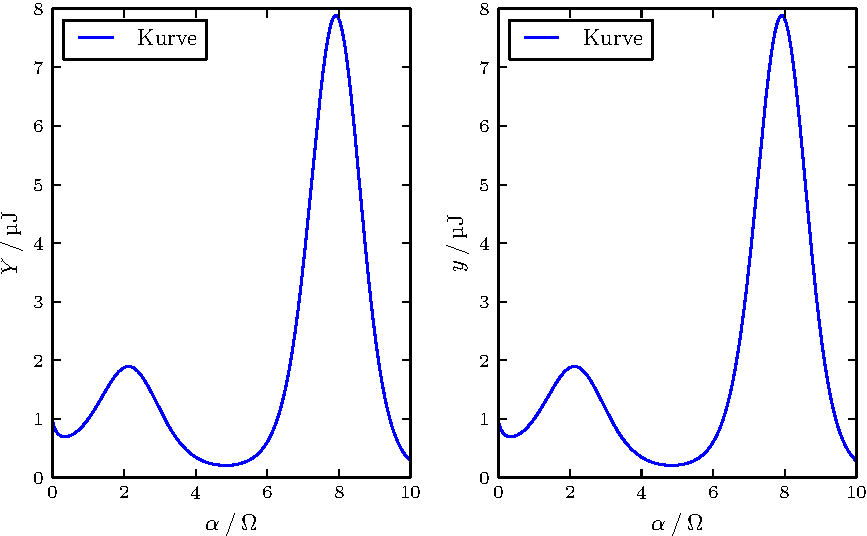
\includegraphics[draft]{plots/plot.pdf}
  \caption{Plot.}
  \label{fig:plot}
\end{figure}

\section{Diskussion}
\label{sec:Diskussion}
\subsection{Diskussion des Aufbaus}
Anstelle einer spektralen Halogen-Lampe kann ein geeignetes  monochromatisches Lasersystem im infraroten Bereich benutzt werden.
Dabei entfällt das Filtern der Wellenlänge.
Dieses Licht kann auf den Lichtzerhacker annähernd punktförmig fokussiert werden, sodass ein klares Rechteck-Signal entsteht.
Das Messsignal lässt sich durch einen Lock-In-Verstärker wegen des zusätzlichen Unterdrückens von frequenzfremden Rauschen besser auswerten als durch den hier benutzten Selektivverstärker.

Die Unsicherheiten in dem Magnetfeld könnten dadurch entstanden sein, dass die Hallsonde zum Messen des Feldes empfindlich auf Änderungen der Ausrichtung reagiert und die Hallsonde nicht fest eingespannt wurde.
Die Stromquelle versorgte den Magneten mit Strom, der über den gesamten Versuch nicht konstant ist, sondern leicht abnimmt.
Das Magnetfeld nahm also im Laufe der Messungen leicht ab, welches in der Rechnung nicht berücksichtigt wurde.
Durch diese mangelnde Präzision der Magnetfeldstärke schlagen sich in Gleichung \eqref{eqn:formel} mit linearer Abhängigkeit Messfehler nieder.

\subsection{Diskussion der Methode und Aussagekraft der Messergebnisse}
Werden die Werte für die Differenzwinkel graphisch gegen $\lambda²$ aufgetragen, lässt sich erkennen, dass diese von der Geraden weit entfernt sind. Dies spricht für eine mangelhafte Messmethode.

Durch starkes Rauschen ist das Finden des Endsignal-Minimums am Oszilloskop schwer. Es kann also nur mit geringer Genauigkeit eine Aussage über die effektive Masse getroffen werden.
Allerdings sind die erhaltenen Werte der effektiven Elektronmasse recht nah am Literaturwert von $m_* = \SI{0.067}{m_e}$ \cite{Hurensohn3}, sodass die systematischen Fehler aus der Messapparatur weniger ins Gewicht fallen als erwartet.


\printbibliography

\section{Anhang}
\begin{figure}[p]
  \centering
\begin{subfigure}{0.7\textwidth}
  \centering
  \includegraphics[width=\textwidth]{pc/brass.pdf}
\end{subfigure}
\begin{subfigure}{0.7\textwidth}
  \centering
  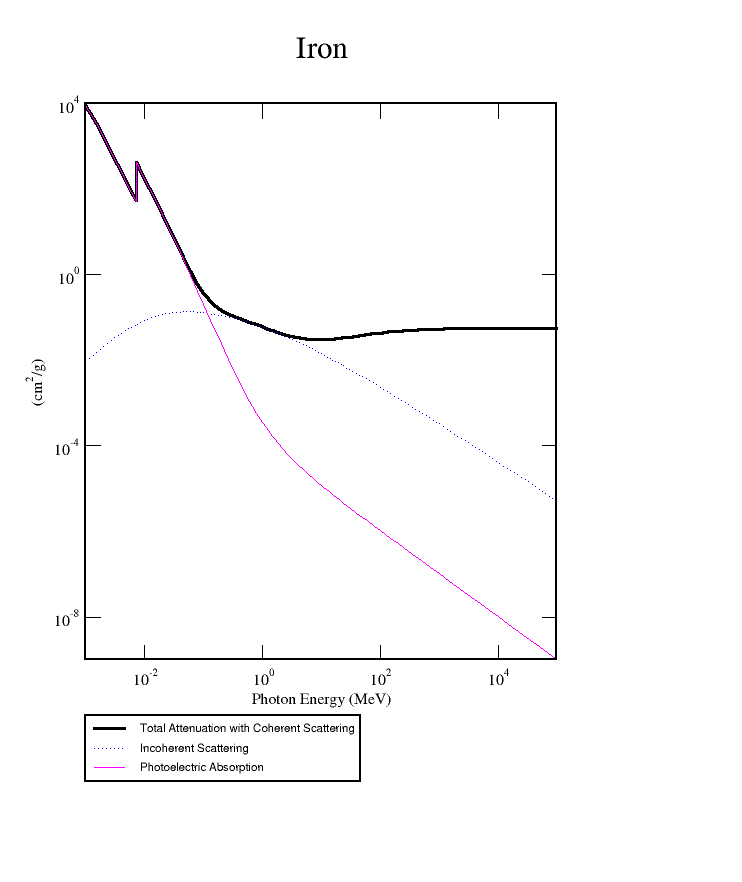
\includegraphics[width=\textwidth]{pc/iron.pdf}
\end{subfigure}
\begin{subfigure}{0.7\textwidth}
  \centering
  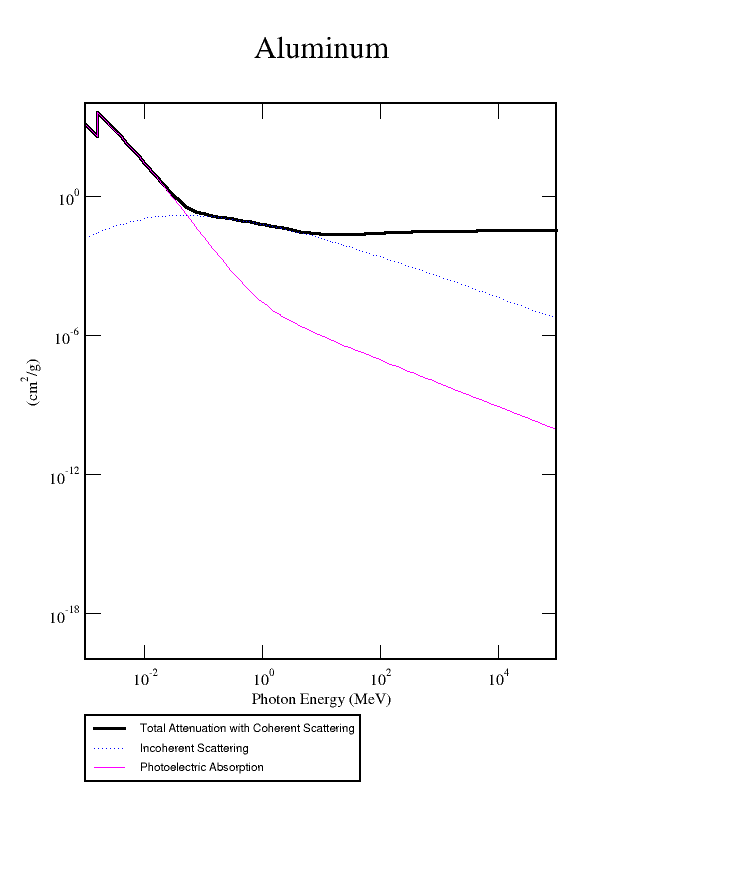
\includegraphics[width=\textwidth]{pc/aluminum.pdf}
\end{subfigure}
\end{figure}
\begin{figure}[p]
  \centering
\begin{subfigure}{0.7\textwidth}
  \centering
  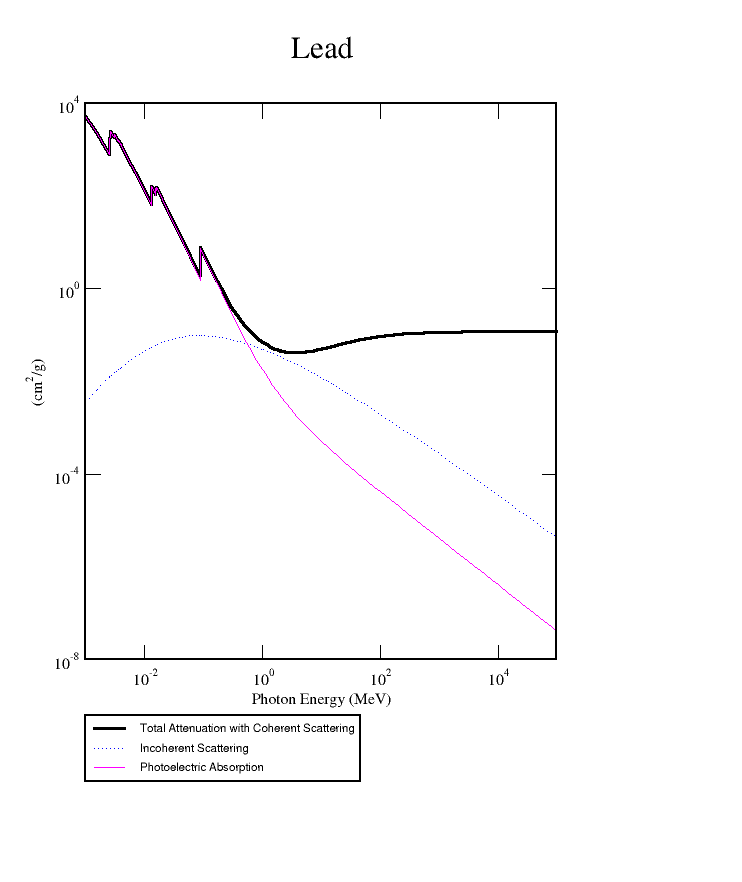
\includegraphics[width=\textwidth]{pc/lead.pdf}
\end{subfigure}
\centering
\begin{subfigure}{0.7\textwidth}
  \centering
  \includegraphics[width=\textwidth]{pc/pom.pdf}
\end{subfigure}
\end{figure}

\end{document}
